% --- Distributed inference ---
\begin{frame}{Serving Is Not Training}
  \begin{itemize}\itemsep0.35em
    \item[\textcolor{red}{$\blacktriangleright$}] Three of the four memory terms simply vanish at inference: no gradients, no optimizer moments, no master weights. \textbf{$16\Psi$ becomes $2\Psi$.}
    \item[\textcolor{red}{$\blacktriangleright$}] But the workload inverts in three ways that change every design decision:
      \begin{itemize}\itemsep0.2em\footnotesize
        \item \textbf{One long job becomes many short ones.} Training is a single synchronous job over all ranks; serving is millions of independent requests with individual latency targets.
        \item \textbf{A new state appears.} The KV cache grows with every generated token and is \emph{per request}, not per model.
        \item \textbf{The bottleneck moves.} Decode reads the whole weight matrix to produce one token, so it is memory-bandwidth-bound rather than compute-bound.
      \end{itemize}
    \item[\textcolor{red}{$\blacktriangleright$}] \textbf{Scope.} Deck 17 owns the single-node story --- KV caching, continuous batching, PagedAttention, speculative decoding, quantization, distillation, and pruning. This section covers only what changes when the deployment spans \emph{several GPUs or several nodes}.
    \item[\textcolor{red}{$\blacktriangleright$}] The multi-GPU question has exactly two answers, and real deployments use both at once: \textbf{replicate} the model, or \textbf{shard} it.
  \end{itemize}
\end{frame}

\begin{frame}{Replication Versus Tensor-Parallel Serving}
  \centering
  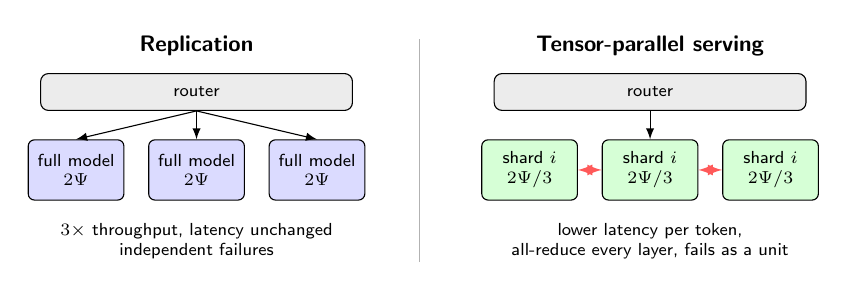
\begin{tikzpicture}[font=\sffamily\scriptsize, >=latex, scale=0.9,
      every node/.style={transform shape},
      gpu/.style={draw, rounded corners=0.08cm, minimum width=1.35cm, minimum height=0.85cm, align=center},
      rt/.style={draw, fill=gray!15, rounded corners=0.1cm, minimum width=4.4cm, minimum height=0.52cm}]
    % Left: replication
    \node[font=\sffamily\small\bfseries] at (2.2,2.5) {Replication};
    \node[rt] (r1) at (2.2,1.85) {router};
    \foreach \i/\x in {0/0.5, 1/2.2, 2/3.9} {
      \node[gpu, fill=blue!14] (a\i) at (\x,0.75) {full model\\$2\Psi$};
      \draw[->] (r1.south) -- (a\i.north);
    }
    \node[font=\sffamily\scriptsize, align=center] at (2.2,-0.25) {$3\times$ throughput, latency unchanged\\independent failures};
    % Divider
    \draw[black!30] (5.35,-0.55) -- (5.35,2.6);
    % Right: tensor parallel
    \node[font=\sffamily\small\bfseries] at (8.6,2.5) {Tensor-parallel serving};
    \node[rt] (r2) at (8.6,1.85) {router};
    \foreach \i/\x in {0/6.9, 1/8.6, 2/10.3} {
      \node[gpu, fill=green!16] (b\i) at (\x,0.75) {shard $i$\\$2\Psi/3$};
    }
    \draw[->] (r2.south) -- (b1.north);
    \draw[<->, thick, red!65] (b0.east) -- (b1.west);
    \draw[<->, thick, red!65] (b1.east) -- (b2.west);
    \node[font=\sffamily\scriptsize, align=center] at (8.6,-0.25) {lower latency per token,\\all-reduce every layer, fails as a unit};
  \end{tikzpicture}
  \vspace{0.5em}
  \begin{itemize}\footnotesize\itemsep0.2em
    \item[\textcolor{red}{$\blacktriangleright$}] \textbf{Replicate when the model fits.} $N$ replicas give $N\times$ throughput at unchanged per-request latency, and each replica fails independently. This is the cheapest and most robust axis --- always exhaust it first.
    \item[\textcolor{red}{$\blacktriangleright$}] \textbf{Shard when it does not, or when latency matters.} Because decode is bandwidth-bound, splitting the weights across $t$ GPUs also splits the bytes each GPU must read per token, so tensor parallelism genuinely reduces time-per-output-token --- not merely memory.
    \item[\textcolor{red}{$\blacktriangleright$}] The cost is two all-reduces per layer \emph{per generated token}, on the critical path. The same NVLink rule applies: \textbf{keep the tensor-parallel group inside one node}. vLLM's guidance is TP $=$ GPUs per node, PP $=$ number of nodes.
  \end{itemize}
\end{frame}

\begin{frame}[allowframebreaks]{The KV Cache Is the Real Constraint}
  \begin{itemize}\footnotesize\itemsep0.3em
    \item[\textcolor{red}{$\blacktriangleright$}] Weights are a fixed cost paid once. The KV cache is a \emph{per-request} cost that grows with every token, and it is what actually caps concurrency.
    \item[\textcolor{red}{$\blacktriangleright$}] Per token, per layer, the cache holds a key and a value for each KV head:
      \[
        \text{bytes} = 2 \times n_{kv} \times d_{\text{head}} \times \text{bytes per element}.
      \]
    \item[\textcolor{red}{$\blacktriangleright$}] \textbf{Worked example --- a 70B model with grouped-query attention} ($L = 80$ layers, $n_{kv} = 8$, $d_{\text{head}} = 128$, \texttt{bf16}), served with $t = 4$ on 4$\times$80\,GB:
      \begin{itemize}\itemsep0.15em\footnotesize
        \item Per token per layer: $2 \times 8 \times 128 \times 2 = 4096$ bytes.
        \item Per token, all layers: $4096 \times 80 = 327{,}680$ bytes $\approx 0.33$\,MB.
        \item An 8192-token conversation: $0.33\,\text{MB} \times 8192 \approx \mathbf{2.7\ GB}$ --- for \emph{one} request.
        \item Budget: $4 \times 80 = 320$\,GB total, minus $140$\,GB of weights and roughly $20$\,GB of workspace leaves $\approx 160$\,GB, so about \textbf{60 concurrent 8k-token sessions}.
      \end{itemize}
    \item[\textcolor{red}{$\blacktriangleright$}] Three consequences that are easy to miss:
      \begin{itemize}\itemsep0.15em\footnotesize
        \item Tensor parallelism shards the \emph{KV heads} too, so it raises the aggregate cache budget as well as splitting the weights.
        \item Without GQA this model would need $64$ KV heads instead of $8$ --- $8\times$ the cache, or roughly 7 concurrent sessions instead of 60.
        \item Replicas do \emph{not} share a KV cache. Adding replicas multiplies capacity but never pools it.
      \end{itemize}
  \end{itemize}
\end{frame}

\begin{frame}[allowframebreaks]{Routing: the Scheduler Above the Replicas}
  \begin{itemize}\itemsep0.4em
    \item[\textcolor{red}{$\blacktriangleright$}] With $N$ replicas you need a router, and the naive choices are all wrong. \textbf{Round-robin fails} because request cost varies by orders of magnitude: a 200-token completion and a 100k-token document summary are not interchangeable units of work.
    \item[\textcolor{red}{$\blacktriangleright$}] \textbf{Route on state, not on count.} The useful signals are queue depth, the number of active sequences, and --- most importantly --- how much KV cache each replica has left. A replica with free HBM can absorb a new request; one at 95\% cache occupancy will start preempting.
    \item[\textcolor{red}{$\blacktriangleright$}] \textbf{Prefix-cache-aware routing} is the highest-value addition in practice. Requests that share a long system prompt or a document prefix should land on the \emph{same} replica, where that prefix is already in the KV cache. Hashing on the prompt prefix can turn a full prefill into a cache hit.
    \item[\textcolor{red}{$\blacktriangleright$}] \textbf{Prefill/decode disaggregation} takes this one step further. The two phases have opposite bottlenecks --- prefill is compute-bound, decode is memory-bandwidth-bound --- and colocating them makes each interfere with the other. DistServe assigns them to \emph{different} GPU pools with independently chosen parallelism, then ships the KV cache between them, reporting \textbf{7.4$\times$ more requests or 12.6$\times$ tighter latency targets}; Splitwise makes the same split across differently specified hardware.
    \item[\textcolor{red}{$\blacktriangleright$}] Continuous batching and PagedAttention (deck 17) operate \emph{within} a replica; routing and disaggregation operate \emph{across} them. Both are needed, and neither substitutes for the other.
  \end{itemize}
  \vspace{0.1em}
  {\scriptsize Zhong et al., ``DistServe,'' OSDI 2024, \href{https://arxiv.org/abs/2401.09670v3}{arXiv:2401.09670v3}; Patel et al., ``Splitwise,'' ISCA 2024, \href{https://arxiv.org/abs/2311.18677v2}{arXiv:2311.18677v2}.}
\end{frame}

\begin{frame}{Failure Handling: Two Very Different Problems}
  \begin{columns}[T,onlytextwidth]
    \column{0.48\textwidth}
      \textbf{Training: all-or-nothing}
      \begin{itemize}\scriptsize\itemsep0.05em
        \item[\textcolor{red}{$\blacktriangleright$}] Every collective is a barrier, so \textbf{one dead rank kills the step} --- and with it the whole job.
        \item[\textcolor{red}{$\blacktriangleright$}] Recovery means restarting from the last checkpoint, so checkpoint frequency directly bounds the work you can lose.
        \item[\textcolor{red}{$\blacktriangleright$}] This is not a rare-event concern at scale. Meta's Llama 3 405B run on 16{,}384 H100s logged \textbf{419 unexpected interruptions in 54 days} --- roughly one every three hours --- with about 78\% traced to hardware, GPUs alone accounting for 58.7\%.
        \item[\textcolor{red}{$\blacktriangleright$}] Mitigations: asynchronous sharded checkpointing, elastic launchers with automatic restarts, health checks that eject a bad node before it corrupts a step, and hot spare nodes.
      \end{itemize}
    \column{0.48\textwidth}
      \textbf{Serving: degrade, do not die}
      \begin{itemize}\scriptsize\itemsep0.05em
        \item[\textcolor{red}{$\blacktriangleright$}] The unit of failure is a \textbf{replica}, and a tensor-parallel group is one replica: lose a single GPU and the whole group goes down.
        \item[\textcolor{red}{$\blacktriangleright$}] So a wider tensor-parallel degree is a \emph{worse} availability story. Prefer the smallest $t$ that meets your latency target, and get throughput from replicas.
        \item[\textcolor{red}{$\blacktriangleright$}] In-flight requests on a failed replica are lost. Their KV cache is not replicated anywhere --- and replicating it would cost more than re-running the prefill.
        \item[\textcolor{red}{$\blacktriangleright$}] Mitigations: health probes, drain-then-restart on deploys, request-level retries with idempotent semantics, and capacity headroom so the survivors absorb the load.
      \end{itemize}
  \end{columns}
  \vspace{0.12em}
  \begin{itemize}\scriptsize
    \item[\textcolor{red}{$\blacktriangleright$}] The asymmetry is worth stating plainly: \textbf{training optimises for progress, serving optimises for availability.} That is why training tolerates deep parallelism and serving does not.
  \end{itemize}
  \vspace{0.03em}
  {\scriptsize Llama Team, AI @ Meta, ``The Llama 3 Herd of Models,'' \href{https://arxiv.org/abs/2407.21783v3}{arXiv:2407.21783v3}, Section 3.3.4 (Reliability and Operational Challenges).}
\end{frame}
